\subsection*{PIC-Programmierung Übungsaufgabe Nr 1}
\subsubsection*{Aufgabe:}
An einer Kegelbahn sollen die geworfenen Kegel als Zahlenwert angezeigt
werden. In einem Unterprogramm werden dazu die liegenden Kegel
gezählt und als BCD-Wert im W-Register dem Hauptprogramm
zurückgegeben. Das Hauptschleife des Hauptprogramms besteht nur aus
dem Unterprogrammaufruf. Eine Ausgangroutine ist nicht vorgesehen.
\subsubsection*{Hardwarebeschreibung:}
Jeder Kegel, der richtig steht, schließt einen Schaltkontakt gegen Masse.
Fällt der Kegel, liefert der entsprechende Kontakt somit ein High-Signal
\begin{figure}[H]
    \centering
    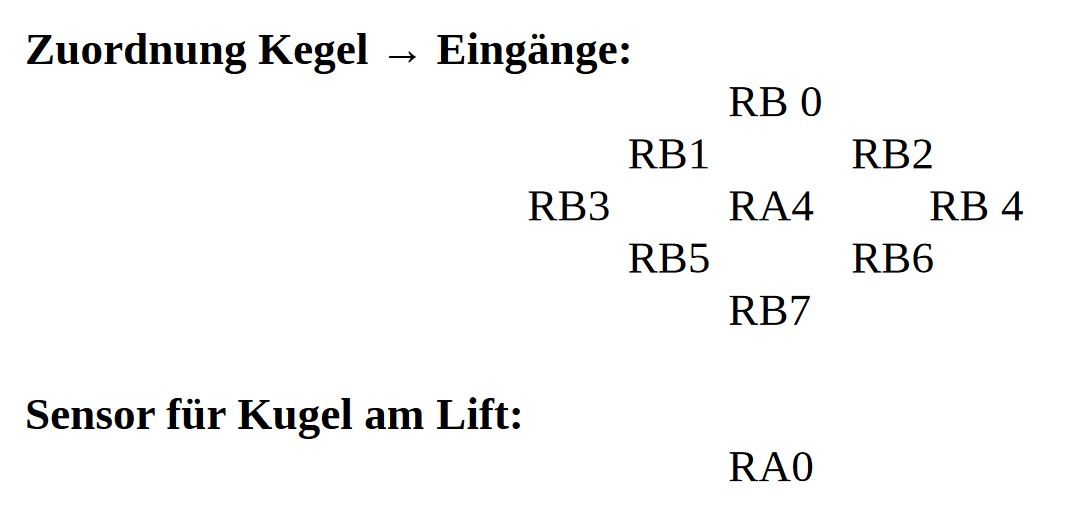
\includegraphics[width=10cm]{inputs/Kegel-Aufgabe.jpg}
    
\end{figure}
\begin{lstlisting}[language=avr]
Start
    BSF     status, rp0
    MOVLW   255
    MOVWF   06/trisb
    MOVLW   255
    MOVWF   trisa
    BCF     status, rp0
    GOTO    Hauptprogramm

Hauptprogramm
    CALL    Unterprogramm
    GOTO    Hauptprogramm

Unterprogramm
    CLRF    counter
    BTFSC   RA0
    RETLW   0
    BTFSC   RA4
    INCF    counter
    MOVLW   8
    MOVWF   loopCnt

Schleife
    BTFSC   RB, 0
    INCF    counter
    RRF     RB
    DECFSZ  loopCnt
    GOTO    Schleife

    MOVF    counter, W
    RETURN
\end{lstlisting}